% 本文件是示例论文的一部分
% 论文的主文件位于上级目录的 `main.tex`

\chapter{粮食生产模型的建立与分析}

本章主要介绍全文建立的基于粗糙集方法的粮食生产模型,包括研究数据、模型框架、模型方法(特征选择方法、预测模型方法等)
\section{粮食生产数据}
\subsection{研究对象}
根据引言所述,本文选择了我国在2022年受到俄乌冲突影响最大的代表性主要农作物—玉米作为研究对象,通过利用粗糙集与其他经典特征选择方法筛选出影响其产量的主要影响因素,进而对我国农作物的生产与规划做出分析与建议。
\subsection{数据来源}
本文研究数据分别参考了《全国农产品成本收益资料汇编》与《中国农村统计年鉴》中各省农作物的生产数据与农村社会经济生产数据。其中在《全国农产品成本收益资料汇编》中选取了各省玉米历年与生产相关的生产数据,如每亩化肥用量、每亩种子用量等,反映的是作物在生产过程中的资源投入情况。在《中国农村统计年鉴》中选取了各省历年农村基本情况与生产状况的数据,如各省农业机械总动力、各省受灾面积等,反映的是各省农村生产条件与状况。
\subsection{数据范围}
本文研究数据在时间尺度上选择了《全国农产品成本收益资料汇编》与《中国农村统计年鉴》在2004-2021年的数据,空间尺度上选择了以上两个数据集中关于玉米生产所共有的19个主要农业大省的数据,具体见下表:
\[
\text{空间尺度}
\begin{cases}
\text{东北地区:辽宁、吉林、黑龙江}\\
\text{华北地区:河北、山西、内蒙古}\\
\text{华东地区:江苏、安徽、山东}\\
\text{中南地区:河南、湖北}\\
\text{西南地区:四川、重庆、贵州、云南}\\
\text{西北地区:陕西、甘肃、宁夏、新疆}
\end{cases}
\]

\begin{figure}[htbp]
  \centering
  \resizebox{\textwidth}{!}
  {
  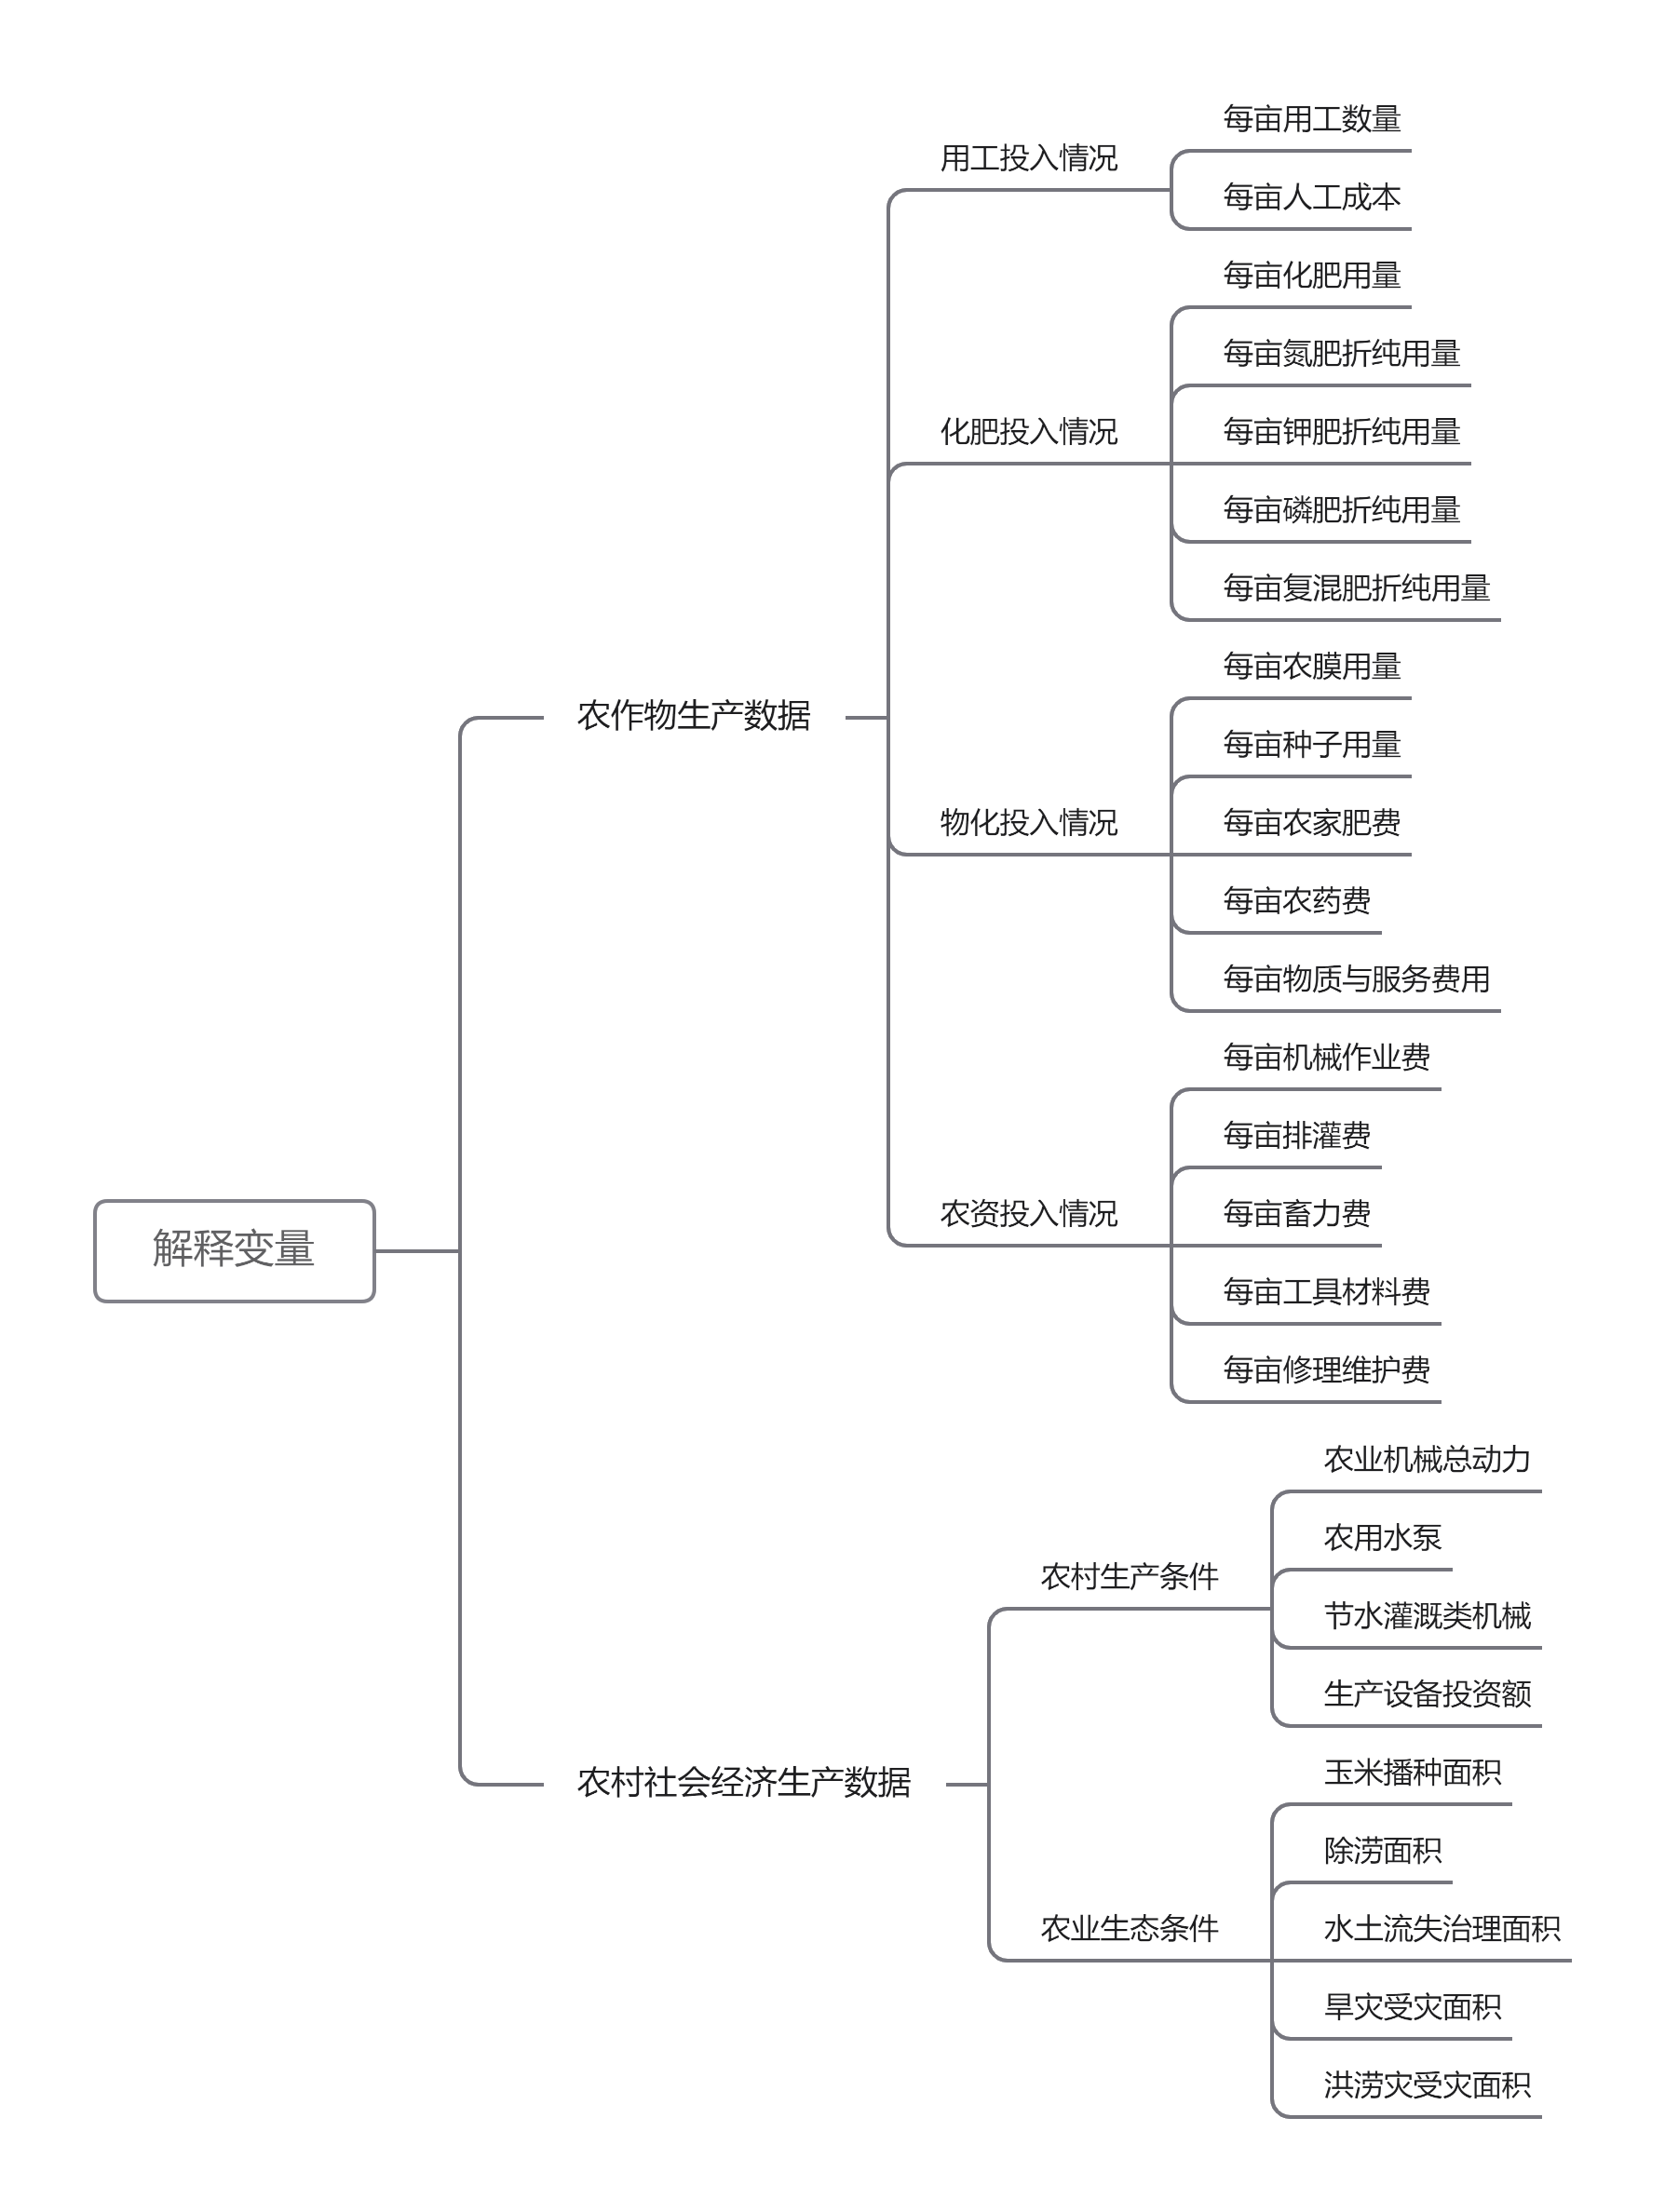
\includegraphics{figs/explanatory_variable.png}
  }
  \caption{26个玉米生产解释变量}
  \label{fig:explanatory_variable}
\end{figure}


\subsection{研究变量}
本文研究中,被解释变量选为各省历年每亩玉米的产量,解释变量共计26个,分别选自《全国农产品成本收益资料汇编》与《中国农村统计年鉴》中与作物生产相关的各方面数据,其中《全国农产品成本收益资料汇编》中选择的解释变量均为各省历年仅投入到每亩玉米土地的数据,而非所有粮食作物的宏观统计数据,所有解释变量见\ref{fig:explanatory_variable}。


% \[
% \text{解释变量}
% \begin{cases}
% \text{  农作物生产数据  }
% \begin{cases}
%   \text{用工投入情况}
%   \begin{cases}
%     \text{每亩用工数量}\\
%     \text{每亩人工成本}
%   \end{cases}\\
%   \text{化肥投入情况}
%   \begin{cases}
%     \text{每亩化肥用量}\\
%     \text{每亩氮肥折纯用量}\\
%     \text{每亩钾肥折纯用量}\\
%     \text{每亩磷肥折纯用量}\\
%     \text{每亩复混肥折纯用量}\\
%   \end{cases}\\
%   \text{物化投入情况}
%   \begin{cases}
%     \text{每亩农膜用量}\\
%     \text{每亩种子用量}\\
%     \text{每亩农家肥费}\\
%     \text{每亩农药费}\\
%     \text{每亩物质与服务费用}
%   \end{cases}\\
%   \text{农资投入情况}
%   \begin{cases}
%     \text{每亩机械作业费}\\
%     \text{每亩排灌费}\\
%     \text{每亩畜力费}\\
%     \text{每亩工具材料费}\\
%     \text{每亩修理维护费}\\
%   \end{cases}\\
%   \end{cases}\\
% \text{农村社会经济生产数据}
% \begin{cases}
% \text{农村生产条件}
% \begin{cases}
%   \text{农业机械总动力}\\
%   \text{农用水泵}\\
%   \text{节水灌溉类机械}\\
%   \text{生产设备投资额}\\
% \end{cases}\\
% \text{农业生态条件}
% \begin{cases}
%   \text{玉米播种面积}\\
%   \text{除涝面积}\\
%   \text{水土流失治理面积}\\
%   \text{旱灾受灾面积}\\
%   \text{洪涝灾受灾面积}\\
% \end{cases}
% \end{cases}
% \end{cases}
% \]




% \DTLloaddb{Data}{data/Data.csv}
% \begin{table}[htbp]
%       \centering
%       \caption{玉米生产数据:陕西省}
%       \label{table:Data}
%       \resizebox{\textwidth}{!}
%       {
%       \csvautobooktabular{data/Data.csv}
%       }
% \end{table}

\subsection{数据预处理}
\label{subsection:DataCleaning}
在本文的研究中,对于某些省份个别年份中出现的空值数据选择了零值填充法进行填充。同时为了构造模糊环境,选择了大多数研究中采取的线性函数归一化方法对数据进行预处理\cite{BestOverview},以便后续利用模糊粗糙集属性约简算法进行特征选择。
\section{粮食生产模型}
本节主要介绍本文建立的粮食生产模型,以便能够利用粮食生产模型对粮食安全进行分析。
\subsection{模型框架}
本模型主要由三个主体部分组成,第一部分为特征选择模型,第二部分为预测模型,第三部分对粮食安全进行可视化分析。第一部分的特征选择模型主要用于对解释变量进行筛选,以便得出最重要的解释变量;第二部分的预测模型主要用于对第一部分特征选择模型的结果进行评估与实验分析,以便分析粗糙集方法相对于其他经典特征选择方法的优劣;第三部分对模糊粗糙集属性约简算法得到的结果进行可视化分析,以便对我国玉米生产及粮食安全提供建议。模型框架见\ref{fig:FoodProductionModel}。


\begin{figure}[htbp]
  \centering
  \resizebox{\textwidth}{!}
  {
  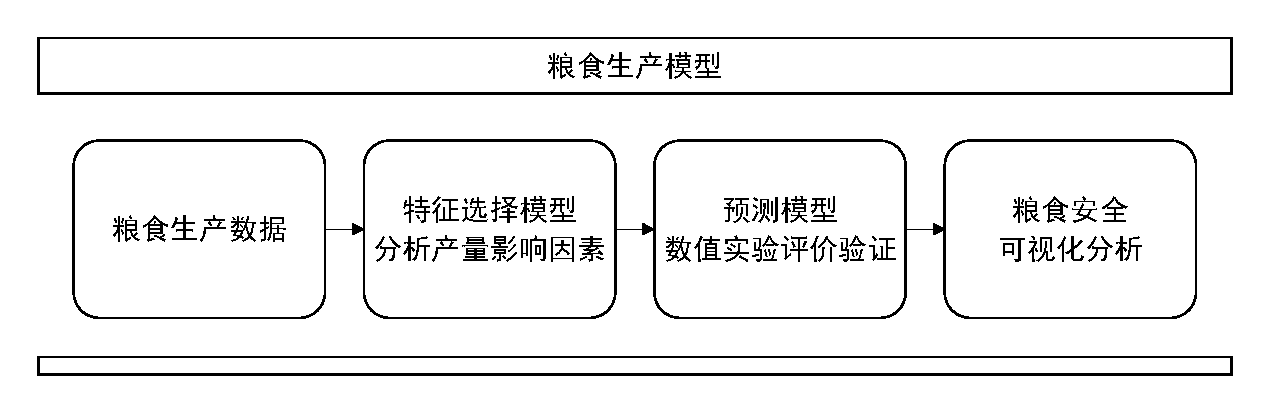
\includegraphics{figs/FoodProductionModel}
  }
  \caption{粮食生产模型框架}
  \label{fig:FoodProductionModel}
\end{figure}


\subsection{特征选择模型}
特征选择模型分别利用了三种不同的特征选择方法:基于属性重要度的模糊粗糙集属性约简算法、基于回归模型的Lasso特征选择算法、基于随机森林模型的随机森林变量重要性算法,通过分别利用以上三种特征选择方法对数据进行特征选择,分别得出不同方法下最重要的10个解释变量,然后再分别将原数据集按照不同特征选择方法得出的特征选择结果进行属性约简,删掉不同方法下重要性排名不在前10的解释变量,分别得到经过三种不同特征选择方法处理后的约简数据集,其中约简后的数据集中只保留了不同特征选择方法下最重要的10个解释变量,以期能够达到在保持分类能力不变的情况下尽可能约简数据集的目的。

\subsection{预测模型}
预测模型在特征选择模型的基础上,通过将不同特征选择模型处理后的约简数据集以及未约简数据集放入预测模型进行预测,以便比较不同数据集在训练误差、训练时间、测试误差、预测精度方面的优劣,进而分析出不同特征选择方法在特征选择方面的差异。

在具体数值实验中,本文选择利用随机森林模型作为预测模型,将各省2004-2020年的约简数据集作为训练数据对模型进行训练,再将各省2021年的粮食单产产量作为预测数据,通过比较预测产量与真实产量之间的差距,进而评估该数据集的预测精度。然而由于预测模型为随机森林模型,理论上特征选择方法中的随机森林变量重要性算法得到的约简数据集对于随机森林预测模型的拟合效果是最好的,因而其在误差、耗时、精度等各方面表现应该较优,因而可以将随机森林变量重要性算法得到的结果作为一个统一的参考,进而可以比较出Lasso算法和粗糙集算法的效果。

\subsection{粮食安全分析}

针对特征选择与预测模型的结果,采用FRAR作为特征选择方法,得到每个省份影响玉米产量的前10个解释变量。并针对相对较为重要的变量从化肥投入情况、成本投入情况、排灌建设情况及机械化建设情况4个方面分别进行了结果可视化,并对特征选择结果进行了分析,为我国玉米生产与粮食安全提供了建议。

%%%%%%%%%%%%%%%%%%%%%%%%%%%%%%%%%%%%%%%%%%%%%%%%%%%%%%%%%%%%%%%%%%%%%%
% \section{插图}

% \subsection{直接插图}
% 使用xelatex命令编译时,\LaTeX{}支持\verb|.pdf|和\verb|.eps|格式的矢量图,
% 也支持\verb|.jpg|、\verb|.png|或\verb|.bmp|格式的位图,当然也可以在\LaTeX{}
% 中直接绘图,关于插图图片推荐的方式有:

% \begin{enumerate}
% \item 使用其它绘图工具绘图生导出或打印成 \verb|pdf| 格式的\emph{矢量图}。
% \item 使用\LaTeX{}的宏包来绘制插图,如 \pkg{Ti\textit{k}Z},它兼容所有 \LaTeX{} 环境,
% 字体能与全文统一,质量最佳,但是需要的学习成本较大。
% 请务必先阅读 \pkg{Ti\textit{k}Z} 文档教程,
% 然后可以去 texample\footnote{\url{http://texample.net/tikz}} 等网站上找类似的例子,
% \item 利用截图工具生成位图,不过\emph{质量堪忧},小心遭批。
% \item 对于现场照片等只能用相机等设备拍照成位图插入,小心遭批。
% \item 最后,一般论文都是\emph{单色印刷}的,请确保插图在黑白打印情况下的清晰度。
% \end{enumerate}

% % \begin{figure}[!htb]
% %   \centering
% %   \newcounter{density}
% %   \setcounter{density}{20}
% %   \begin{tikzpicture}[font=\small]
  \def\couleur{orange}
  \path[coordinate] (0,0) coordinate(A)
              ++( 90:4cm) coordinate(B)
              ++(0:4cm) coordinate(C)
              ++(-90:4cm) coordinate(D);
  \draw (A) node[left] {A}
    (B) node[left] {B}
    (C) node[right] {Point C} --
    (D) node[right,midway,align=left] {边长$a$ \\ 面积和:$S=\frac{50}{9}a^2$ \\ 边长和:$C=\frac{20}{9}(10+\sqrt{82})a$}
    node[right] {点D};
  \draw[fill=\couleur!\thedensity] (A)--(B)--(C)--(D)--cycle;
  \foreach \x in {1,...,40}{%
      \pgfmathsetcounter{density}{\thedensity+25}
      \setcounter{density}{\thedensity}
      \path[coordinate] coordinate(X) at (A){};
      \path[coordinate] (A) -- (B) coordinate[pos=.1](A)
                          -- (C) coordinate[pos=.1](B)
                          -- (D) coordinate[pos=.1](C)
                          -- (X) coordinate[pos=.1](D);
      \draw[fill=\couleur!\thedensity] (A)--(B)--(C)--(D)--cycle;
  }
\end{tikzpicture}

% %   \caption{在\LaTeX{}中直接用Ti\textit{k}Z绘制的矢量图}
% %   \label{fig:tikzrot}
% % \end{figure}

% \begin{figure}[!htb][H]
%   \centering
%   
\includegraphics[width=4.1cm]{nwafu-circle}
%   \caption{CorelDraw绘制导出的校徽PDF矢量图}
%   \label{fig:logo}
% \end{figure}


% \subsection{子图排版}

% 如需要多个子图共用一个题注,需加载额外宏包,可以使用\pkg{subcaption}等宏包实现,
% 如\autoref{fig:sub2}所示。若需要更为复杂的子图控制,个人推荐使用\pkg{floatrow}
% 宏包实现更为复杂和灵活的子图排版中的细节控制。

% \begin{figure}[!htb]
%   \centering
%   \subfloat[左边的大校徽\label{fig:sub1}]{
%     
\includegraphics[width=2.8cm]{nwafu-circle}
%   }\quad
%   \subfloat[短标题:小校徽][小校徽,题注很长,不过请各位放心,它会自动换行\label{fig:sub2}]
%   {
%     
\includegraphics[width=4.6cm]{nwafu-bar}
%   }
%   \caption{用subcaption宏包排版子图}
%   \label{fig:subfigs}
% \end{figure}

% 强烈建议使用\emph{矢量图}图片,获得矢量图的一种方式是是直接使用
% \LaTeX{}的绘制宏包\pkg{Ti\textit{k}Z}、\pkg{pgfplots}等宏包进行绘制,另一
% 种获取矢量图的方式是用Matplotlib、MatLab、Mathematica、Python等工具绘图后
% 导出pdf格式的矢量图。如\ref{fig:plots}所示。

% \begin{figure}[htb]
%   \centering
%   \subfloat[二维图像\label{fig:func}]
%     {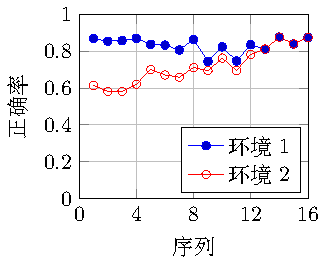
\includegraphics[scale=0.65]{figs/plot_2d}} \qquad
%   \subfloat[三维图像\label{fig:sum}]
%     {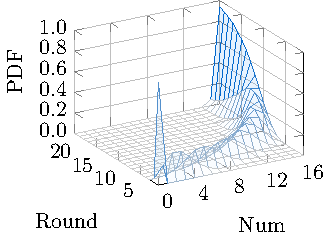
\includegraphics[scale=0.65]{figs/plot_3d}}
%   \caption{利用 \pkg{pgfplot} 绘图}
%   \label{fig:plots}
% \end{figure}
% %

% \subsection{双语题注排版}

% 在研究生学位论文中,需使用双语题注(中文和英文),为此,本模板选用
% \pkg{bicaption}宏包实现双语题注,其效果可以参考\ref{fig:bicap}。当然,
% 也可以使用其它宏包实现双语题注排版,请大家根据情况自行处理。

% \begin{figure}[!htb]
%   \centering
%   
\includegraphics[width=4.2cm]{nwafu-bar}
%   \bicaption{双语题注}{bilingual caption}
%   \label{fig:bicap}
% \end{figure}

% \subsection{超宽插图排版(卧图)}

% 如果需要插入图片超出了页面宽度,建议使用\emph{卧排}的方式实现排版,一种常
% 用的方式是使用 \pkg{lscape}宏包提供的 \env{landscape}环境进行排版。效果参
% 见\ref{fig:fullpage1}。

% \setcounter{subfigure}{0}
% \begin{landscape}
% \vspace*{\fill} % 填充空白
% \begin{figure}[!hb]
%   \centering
%   \subfloat[First caption\label{fig:fp1}]
%     {
\includegraphics[width=.8\textheight]{nwafu-bar}} \\
%   \subfloat[Second caption]
%     {
\includegraphics[height=2cm]{nwafu-bar}}
%   \caption{用\emph{卧排}实现超宽插图排版}
%   \label{fig:fullpage1}
% \end{figure}
% \vspace*{\fill} % 填充空白
% \end{landscape}

% \section{表格}

% \subsection{内置表格排版环境}

% 对于简单的表格,可以使用\LaTeX{}内置的 \env{tabular} 环境实现排版,
% 如\ref{tab:city}。

% \begin{table}[htb]
%   \centering
%   \caption[城市人口]{城市人口数量排名 (source: Wikipedia)\label{tab:city}}
%   \begin{tabular}{lr}
%     \toprule
%     \multicolumn{1}{c}{城市} & \multicolumn{1}{c}{人口} \\
%     \midrule
%     Mexico City              & 20,116,842               \\
%     Shanghai                 & 19,210,000               \\
%     Peking                   & 15,796,450               \\
%     Istanbul                 & 14,160,467               \\
%     \bottomrule
%   \end{tabular}
% \end{table}

% \note{在学位论文中,表格要求采用三线表},因此,需要使用\pkg{booktabs}宏包
% 提供的\cs{toprule}、\cs{midrule}和\cs{bottomrule}分别绘制表格的顶线、中线
% 和底线。

% \subsection{表格浮动体}

% 由于学位论文中表格数量较多,且表格内容(长度)变化较大,当表格过长(一页内)时,
% 可能会带来分页困难,与插图类似,\LaTeX{}引入的\emph{浮动体}机制,可以使表格
% 脱离上下文,自动布置于合适的位置,从而避免在排版中产生留白问题。对于表格,
% 浮动体是通过\env{table}环境实现的。同时,利用\env{table}环境还能够较好地实
% 现插图编号及交叉引用的自动化。

% \subsection{跨页长表格}

% 如果表格内容很多,导致无法放在一页内的话,则需要用 \env{longtable}宏包实现
% 表格的跨页排版,如\ref{tab:performance}所示(数据来自南京航空航天大学毕业论
% 文\LaTeX{}模板)。

% % 定义表中用到的的宏,以简化表格代码并为后续修改提供统一接口
% \def\tabcaption{实验数据}
% \def\tabheadrow{
%   \multirow{2}{*}{测试程序} & \multicolumn{1}{c}{正常运行} &
%    \multicolumn{1}{c}{同步} & \multicolumn{1}{c}{检查点} &
%    \multicolumn{1}{c}{卷回恢复} & \multicolumn{1}{c}{进程迁移} &
%    \multicolumn{1}{c}{检查点} \\
%    & \multicolumn{1}{c}{时间(s)} & \multicolumn{1}{c}{时间(s)} &
%    \multicolumn{1}{c}{时间(s)} & \multicolumn{1}{c}{时间(s)} &
%    \multicolumn{1}{c}{时间(s)} & \multicolumn{1}{c}{文件(KB)} \\
%  }

% % 定义跨页表续表表题
% \def\ctntabcap{
%    \caption* {表~\thetable\hskip1em 实验数据(续)}\\
%    \addlinespace[-3.0ex]
%  }
% % 定义跨页表命令集合
% \def\ctntabcmd{
%    \ctntabcap\\
%    \toprule
%    \tabheadrow
%    \midrule
%    \endhead
%    \midrule
%    \multicolumn{7}{r}{\small 接下页}\\
%    \endfoot
%    \endlastfoot
%  }

% \begin{longtable}[c]{c*{6}{r}}
%   \caption[实验数据]{\tabcaption}\label{tab:performance}\\
%   \toprule
%   \tabheadrow
%   \midrule
%   \endfirsthead
%   \ctntabcmd
%   CG.A.2 & 23.05 & 0.002 & 0.116 & 0.035 & 0.589 & 32491 \\
%   CG.A.4 & 15.06 & 0.003 & 0.067 & 0.021 & 0.351 & 18211 \\
%   CG.A.8 & 13.38 & 0.004 & 0.072 & 0.023 & 0.210 & 9890 \\
%   CG.B.2 & 867.45 & 0.002 & 0.864 & 0.232 & 3.256 & 228562 \\
%   CG.B.4 & 501.61 & 0.003 & 0.438 & 0.136 & 2.075 & 123862 \\
%   CG.B.8 & 384.65 & 0.004 & 0.457 & 0.108 & 1.235 & 63777 \\
%   MG.A.2 & 112.27 & 0.002 & 0.846 & 0.237 & 3.930 & 236473 \\
%   MG.A.4 & 59.84 & 0.003 & 0.442 & 0.128 & 2.070 & 123875 \\
%   MG.A.8 & 31.38 & 0.003 & 0.476 & 0.114 & 1.041 & 60627 \\
%   MG.B.2 & 526.28 & 0.002 & 0.821 & 0.238 & 4.176 & 236635 \\
%   MG.B.4 & 280.11 & 0.003 & 0.432 & 0.130 & 1.706 & 123793 \\
%   MG.B.8 & 148.29 & 0.003 & 0.442 & 0.116 & 0.893 & 60600 \\
%   LU.A.2 & 2116.54 & 0.002 & 0.110 & 0.030 & 0.532 & 28754 \\
%   LU.A.4 & 1102.50 & 0.002 & 0.069 & 0.017 & 0.255 & 14915 \\
%   LU.A.8 & 574.47 & 0.003 & 0.067 & 0.016 & 0.192 & 8655 \\
%   LU.B.2 & 9712.87 & 0.002 & 0.357 & 0.104 & 1.734 & 101975 \\
%   LU.B.4 & 4757.80 & 0.003 & 0.190 & 0.056 & 0.808 & 53522 \\
%   CG.B.2 & 867.45 & 0.002 & 0.864 & 0.232 & 3.256 & 228562 \\
%   CG.B.4 & 501.61 & 0.003 & 0.438 & 0.136 & 2.075 & 123862 \\
%   CG.B.8 & 384.65 & 0.004 & 0.457 & 0.108 & 1.235 & 63777 \\
%   MG.A.2 & 112.27 & 0.002 & 0.846 & 0.237 & 3.930 & 236473 \\
%   MG.A.4 & 59.84 & 0.003 & 0.442 & 0.128 & 2.070 & 123875 \\
%   MG.A.8 & 31.38 & 0.003 & 0.476 & 0.114 & 1.041 & 60627 \\
%   MG.B.2 & 526.28 & 0.002 & 0.821 & 0.238 & 4.176 & 236635 \\
%   MG.B.4 & 280.11 & 0.003 & 0.432 & 0.130 & 1.706 & 123793 \\
%   LU.A.2 & 2116.54 & 0.002 & 0.110 & 0.030 & 0.532 & 28754 \\
%   LU.A.8 & 574.47 & 0.003 & 0.067 & 0.016 & 0.192 & 8655 \\
%   LU.B.2 & 9712.87 & 0.002 & 0.357 & 0.104 & 1.734 & 101975 \\
%   LU.B.8 & 2444.05 & 0.004 & 0.222 & 0.057 & 0.548 & 30134 \\
%   EP.A.2 & 123.81 & 0.002 & 0.010 & 0.003 & 0.074 & 1834 \\
%   EP.A.8 & 31.06 & 0.004 & 0.017 & 0.005 & 0.073 & 1661 \\
%   EP.B.2 & 495.49 & 0.001 & 0.009 & 0.003 & 0.196 & 2011 \\
%   EP.B.8 & 126.74 & 0.003 & 0.017 & 0.005 & 0.083 & 1656 \\
%   \bottomrule
% \end{longtable}

% \subsection{表格的双语题注}

% 在研究生学位论文中,需使用双语题注(中文和英文),为此,本模板选用
% \pkg{bicaption}宏包实现双语题注,其效果可以参考\ref{tab:bicap}。当然,
% 也可以使用其它宏包实现双语题注排版,请大家根据情况自行处理。

% \begin{table}[htb]
%   \centering
%   \bicaption[城市人口]{城市人口数量排名 (source:
%     Wikipedia)\label{tab:bicap}}{Urban population ranking}
%   \begin{tabular}{lr}
%     \toprule
%     \multicolumn{1}{c}{城市} & \multicolumn{1}{c}{人口} \\
%     \midrule
%     Mexico City              & 20,116,842               \\
%     Shanghai                 & 19,210,000               \\
%     Peking                   & 15,796,450               \\
%     Istanbul                 & 14,160,467               \\
%     \bottomrule
%   \end{tabular}
% \end{table}

% \subsection{超宽表格排版(卧表)}

% 如果需要插入超出页面宽度的表格,可以使用\pkg{lscape}宏包提供的 \env{landscape}
% 环境排版\emph{卧表},效果参见\ref{tab:toowidetab}。

% \begin{landscape}
% \vspace*{\fill} % 填充空白
% \begin{table}[!htb]
%   \centering
%   \caption{Laser specifications}
%   \label{tab:toowidetab}
%   \begin{tabular}{ccccccccc}
%     \toprule
%     Wavelength & Model & Package & Emmitter type & Manufacturer & Power (mW) & Iop (mA) & Ith (mA) & Vop (V)\\
%     \midrule
%     405 & DL-7386-101HG & TO-56 & single & sanyo & 50-70 & 70 & 35 & 4.8\\
%     450 & PL 450 & TO-38 & single & osram & 50-90 & 120 & 30 & 5.5\\
%     638 & ML520G54 & TO-56 & single & mitsubishi & 90-100 & 150 & 50 & 2.7\\
%     655 &  DL-5147-242 & TO-56 & single & sanyo & 30-50 & 80 & 40 & 3.8\\
%     \bottomrule
%   \end{tabular}
% \end{table}
% \vspace*{\fill} % 填充空白
% \end{landscape}

% 如果需要插入超宽超长表格,可以使用\pkg{lscape}宏包提供的 \env{landscape}
% 结合\env{longtable}环境排版\emph{跨页卧表},效果参见\ref{tab:landscapeperformance}。

% \begin{landscape} 
%   \begin{longtable}[c]{c*{6}{r}}
%     \caption[实验数据]{\tabcaption}\label{tab:landscapeperformance}\\
%     \toprule
%     \tabheadrow
%     \midrule
%     \endfirsthead
%     \ctntabcmd
%     CG.A.2 & 23.05 & 0.002 & 0.116 & 0.035 & 0.589 & 32491 \\
%     CG.A.4 & 15.06 & 0.003 & 0.067 & 0.021 & 0.351 & 18211 \\
%     CG.A.8 & 13.38 & 0.004 & 0.072 & 0.023 & 0.210 & 9890 \\
%     CG.B.2 & 867.45 & 0.002 & 0.864 & 0.232 & 3.256 & 228562 \\
%     CG.B.4 & 501.61 & 0.003 & 0.438 & 0.136 & 2.075 & 123862 \\
%     CG.B.8 & 384.65 & 0.004 & 0.457 & 0.108 & 1.235 & 63777 \\
%     MG.A.2 & 112.27 & 0.002 & 0.846 & 0.237 & 3.930 & 236473 \\
%     MG.A.4 & 59.84 & 0.003 & 0.442 & 0.128 & 2.070 & 123875 \\
%     MG.A.8 & 31.38 & 0.003 & 0.476 & 0.114 & 1.041 & 60627 \\
%     MG.B.2 & 526.28 & 0.002 & 0.821 & 0.238 & 4.176 & 236635 \\
%     MG.B.4 & 280.11 & 0.003 & 0.432 & 0.130 & 1.706 & 123793 \\
%     MG.B.8 & 148.29 & 0.003 & 0.442 & 0.116 & 0.893 & 60600 \\
%     LU.A.2 & 2116.54 & 0.002 & 0.110 & 0.030 & 0.532 & 28754 \\
%     LU.A.4 & 1102.50 & 0.002 & 0.069 & 0.017 & 0.255 & 14915 \\
%     LU.A.8 & 574.47 & 0.003 & 0.067 & 0.016 & 0.192 & 8655 \\
%     LU.B.2 & 9712.87 & 0.002 & 0.357 & 0.104 & 1.734 & 101975 \\
%     LU.B.4 & 4757.80 & 0.003 & 0.190 & 0.056 & 0.808 & 53522 \\
%     LU.B.8 & 2444.05 & 0.004 & 0.222 & 0.057 & 0.548 & 30134 \\
%     CG.B.2 & 867.45 & 0.002 & 0.864 & 0.232 & 3.256 & 228562 \\
%     CG.B.4 & 501.61 & 0.003 & 0.438 & 0.136 & 2.075 & 123862 \\
%     CG.B.8 & 384.65 & 0.004 & 0.457 & 0.108 & 1.235 & 63777 \\
%     MG.A.2 & 112.27 & 0.002 & 0.846 & 0.237 & 3.930 & 236473 \\
%     MG.A.4 & 59.84 & 0.003 & 0.442 & 0.128 & 2.070 & 123875 \\
%     MG.A.8 & 31.38 & 0.003 & 0.476 & 0.114 & 1.041 & 60627 \\
%     MG.B.2 & 526.28 & 0.002 & 0.821 & 0.238 & 4.176 & 236635 \\
%     MG.B.4 & 280.11 & 0.003 & 0.432 & 0.130 & 1.706 & 123793 \\
%     MG.B.8 & 148.29 & 0.003 & 0.442 & 0.116 & 0.893 & 60600 \\
%     LU.A.2 & 2116.54 & 0.002 & 0.110 & 0.030 & 0.532 & 28754 \\
%     LU.A.4 & 1102.50 & 0.002 & 0.069 & 0.017 & 0.255 & 14915 \\
%     LU.A.8 & 574.47 & 0.003 & 0.067 & 0.016 & 0.192 & 8655 \\
%     LU.B.2 & 9712.87 & 0.002 & 0.357 & 0.104 & 1.734 & 101975 \\
%     LU.B.4 & 4757.80 & 0.003 & 0.190 & 0.056 & 0.808 & 53522 \\
%     LU.B.8 & 2444.05 & 0.004 & 0.222 & 0.057 & 0.548 & 30134 \\
%     EP.A.2 & 123.81 & 0.002 & 0.010 & 0.003 & 0.074 & 1834 \\
%     EP.A.4 & 61.92 & 0.003 & 0.011 & 0.004 & 0.073 & 1743 \\
%     EP.A.8 & 31.06 & 0.004 & 0.017 & 0.005 & 0.073 & 1661 \\
%     EP.B.2 & 495.49 & 0.001 & 0.009 & 0.003 & 0.196 & 2011 \\
%     EP.B.4 & 247.69 & 0.002 & 0.012 & 0.004 & 0.122 & 1663 \\
%     EP.B.8 & 126.74 & 0.003 & 0.017 & 0.005 & 0.083 & 1656 \\
%     \bottomrule
%   \end{longtable}
% \end{landscape}
% \newpage

% \subsection{表格自动生成}

% 也可以结合在\pkg{csvsimple}、\pkg{pgfplotstable}、\pkg{datatool}等宏包直接
% 使用逗号分隔的CSV文件中的数据生成\LaTeX{}表格。\ref{tab:datatooltab} 是将
% \ref{tab:performance}中的数据存储在db.csv文件后,用\pkg{datatool}宏包实现
% \LaTeX 表格排版的一个例子。

% \DTLloaddb{ltab}{data/db.csv}% 可以在之前任何位置载入数据
% \begin{longtable}[c]{c*{6}{r}}
%   \caption[实验数据]{\tabcaption}\label{tab:datatooltab}\\
%   \toprule
%   \tabheadrow
%   \midrule
%   \endfirsthead
%   \ctntabcmd
%   \DTLforeach*{ltab}{\cola=cola, \colb=colb, \colc=colc, \cold=cold,
%                      \cole=cole, \colf=colf, \colg=colg}%
%         {\DTLiffirstrow{}{\tabularnewline}%
%         \cola & \colb & \colc & \cold & \cole & \colf & \colg}\\ % 数据列位置可任意
%   \bottomrule
% \end{longtable}

% 在论文撰写中,应具备协作意识。排版是\LaTeX{}的事,而处理数据一定是
% Excel等软件、R语言等开发语言的强项。这些数据处理的结果,
% 多数都可以非常方便的转存为逗号分隔的CSV数据文件。利用这个CSV数据实现表
% 格自动排版,让各类软件各负其责,通力合作才是高效工作之道。在一个软件里
% 干所有的事,不是好办法。

% 为减轻负担,在\nwafuthesis 模板并未直接引入这些CSV数据处理宏包,如果使用,
% 则需要手动载入需要的宏包,并通过查阅其使用说明学习宏包使用方法。
% %
% % \section{用\pkg{easyfloats}处理浮动体}
% %
% % 使用\LaTeX{}提供的\env{figure}和\env{table}浮动体环境,可以轻松实现浮动体排版。
% % 但如果使用\pkg{easyfloats}宏包,则可以简化浮动体的语法,如所示。其使用细节可以
% % 参考\url{https://latexstudio.net/index/details/index/mid/1181.html}中译说明。
% %
% % \emph{注意}:\pkg{easyfloats}宏包较新(2020.12.20),需要注意更新宏包,
% % 本示例文档中未给出示例代码。

% \section{用tabularray宏包排版表格}

% \pkg{tabularray} 是基于\LaTeX3设计的宏包,它不依赖其它宏包而实现排版,不仅
% 提供了基本表格排版功能,而且采用简便键值列表方式实现了表格的内容与格式分离。
% 该宏包被称为是新一代的表格排版,具体用法可见宏包的说明文档
% (\url{https://mirrors.cqu.edu.cn/CTAN/macros/latex/contrib/tabularray/tabularray.pdf})。
% 耿楠完成了该说明文档的翻译
% (\url{https://gitee.com/nwafu_nan/tabularray-doc-zh-cn/releases/2022A})。

% \subsection{用\env{tblr}环境排版简单表格}

% 可以使用\pkg{tabularray}宏包提供的\env{tblr}环境排版简单表格,
% 如\ref{tab:tblr} 所示。

% \begin{table}[htb]
%   \caption{用tblr环境排版表格}
%   \label{tab:tblr}
%   \begin{tblr}{
%     colspec = lcccc,
%     cell{1}{1} = {r=2}{}, cell{1}{2,4} = {c=2}{},
%     hline{1,Z} = {1pt, solid},
%     hline{3} = {solid},
%     hline{2} = {2-3}{},
%     hline{2} = {4-5}{},
%     cells = {font=\small},
%   }
%     Sample & I & & II & \\
%     & A & B & C & D \\
%     S1 & 5 & 6 & 7 & 8 \\
%     S2 & 6 & 7 & 8 & 5 \\
%     S3 & 7 & 8 & 5 & 6 \\
%   \end{tblr}
% \end{table}

% \subsection{用\env{longtblr}环境排版跨页长表格}

% 可以使用\pkg{tabularray}宏包的\env{longtblr}环境实现长表格的跨页排版,但由
% 于本模板未对其格式进行详细设置,因此,需要使用其\cs{DefTblrTemplate}等命令
% 设置长表格的排版模式模板,建议将其置于导言区,以统一设置长表格排版格式,
% 然后再使用这些模板排版长表格。如\ref{tab:longtblr}所示。

% \DefTblrTemplate{caption-tag}{default}{表\hspace{0.25em}\thetable}
% \DefTblrTemplate{contfoot-text}{default}{接下页}
% \DefTblrTemplate{caption-sep}{default}{\enskip}
% \DefTblrTemplate{conthead-text}{default}{\!(续)}

% \NewTblrTheme{fancy}{
%   \SetTblrStyle{firsthead,mddlehead,lasthead}{font=\centering\small\sffamily}
%   \SetTblrStyle{firstfoot}{font=\small}
%   \SetTblrStyle{middlefoot}{font=\small}
%   \SetTblrStyle{lastfoot}{font=\small}
% }

% \begin{longtblr}[
%   theme = fancy,
%   caption = {一个长长长长长长长长长的表格},
%   entry = {短标题},
%   label = {tab:longtblr},
%   note{a} = {第一个表注。},
%   note{$\dag$} = {第二个长长长长长长长的表注。},
%   remark{注意} = {一些常规说明,一些常规说明,一些常规说明。},
%   remark{来源} = {自力更生,自力更生,自力更生。},
% ]{
%   colspec = {XXX}, width = 0.85\linewidth,
%   rowhead = 1,
%   hline{1,Z} = {1pt, solid},
%   hline{2} = {solid},
%   cells = {font=\small},
% }
%  Head    & Head  & Head    \\
%  Alpha   & Beta  & Gamma   \\
%  Epsilon & Zeta\TblrNote{a}       & Eta    \\
%  Iota    & Kappa\TblrNote{$\dag$} & Lambda \\
%  Nu      & Xi    & Omicron \\
%  Rho     & Sigma & Tau     \\
%  Phi     & Chi   & Psi     \\
%  Alpha   & Beta  & Gamma   \\
%  Epsilon & Zeta  & Eta     \\
%  Iota    & Kappa & Lambda  \\
%  Nu      & Xi    & Omicron \\
%  Rho     & Sigma & Tau     \\
%  Phi     & Chi   & Psi     \\
%  Alpha   & Beta  & Gamma   \\
%  Epsilon & Zeta  & Eta     \\
%  Iota    & Kappa & Lambda  \\
%  Nu      & Xi    & Omicron \\
%  Rho     & Sigma & Tau     \\
%  Phi     & Chi   & Psi     \\
%  Alpha   & Beta  & Gamma   \\
%  Epsilon & Zeta  & Eta     \\
%  Iota    & Kappa & Lambda  \\
%  Nu      & Xi    & Omicron \\
%  Rho     & Sigma & Tau     \\
%  Phi     & Chi   & Psi     \\
%  Alpha   & Beta  & Gamma   \\
%  Epsilon & Zeta  & Eta     \\
%  Iota    & Kappa & Lambda  \\
%  Nu      & Xi    & Omicron \\
%  Rho     & Sigma & Tau     \\
%  Phi     & Chi   & Psi     \\
% \end{longtblr}


% \subsection{用\env{booktabs}环境三线表}

% 如果在导言区使用\cs{UseTblrLibrary}命令引入\pkg{booktabs},则该宏包可以通
% 过\env{booktabs}更为灵活的实现三线表的排版,如\ref{tab:booktabs}所示。

% \begin{table}[htb]
%   \caption{用tblr环境排版表格}
%   \label{tab:booktabs}
%   \begin{booktabs}{
%     colspec = lcccc,
%     cell{1}{1} = {r=2}{}, cell{1}{2,4} = {c=2}{},
%     cells = {font=\small},
%   }
%     \toprule
%     Sample & I & & II & \\
%     \cmidrule[lr]{2-3} \cmidrule[lr]{4-5}
%     & A & B & C & D \\
%     \midrule
%     S1 & 5 & 6 & 7 & 8 \\
%     S2 & 6 & 7 & 8 & 5 \\
%     S3 & 7 & 8 & 5 & 6 \\
%     \bottomrule
%   \end{booktabs}
% \end{table}

% \section{为表格添加数据来源说明}

% 对于学位论文,往往需要为表格添加数据来源说明及必要的其它注释说明。这可以
% 使用\pkg{tabularray}宏包的\env{longtblr}跨页长表格环境(\ref{tab:longtblr})
% 或\env{talltblr}浮动长表格环境实现,也可以通过\pkg{threeparttable}宏包实现。

% \subsection{用tabularray宏包的talltblr环境添加数据来源说明}

% \pkg{tabularray}宏包的\env{talltblr}环境可以实现可浮动长表格,并可以实现表
% 格题注和尾注排版,从而实现为表格添加数据来源说明,如\ref{tab:talltblr}

% \begin{table}[htp]
%   \begin{talltblr}[
%     theme = fancy,
%     caption = {用talltblr为表格添加脚注说明},
%     entry = {短标题},
%     label = {tab:talltblr},
%     note{a} = {第一个表注。},
%     note{$\dag$} = {第二个长长长长长长长的表注。},
%     remark{注意} = {一些常规说明,一些常规说明,一些常规说明。},
%     remark{来源} = {自力更生,自力更生,自力更生。},
%   ]{
%     colspec = {XXX}, width = 0.8\linewidth,
%     hline{1,Z} = {1pt, solid},
%     hline{2} = {solid},
%     cells = {font=\small},
%   }
%     Alpha   & Beta  & Gamma                   \\
%     Epsilon & Zeta  & Eta\TblrNote{a}         \\
%     Iota    & Kappa & Lambda\TblrNote{$\dag$} \\
%   \end{talltblr}
% \end{table}

% \subsection{用threeparttable宏包添加数据来源说明}
% 该宏包用于为表格添加脚注说明,如\ref{tab:threeparttable}。

% \begin{table}[htp]
%   \caption{用threeparttable为表格添加脚注说明}
%   \label{tab:threeparttable}
%   \begin{threeparttable}
%     \begin{tabular}{c c c c}
%       \toprule
%       1st Column & 2nd Colimn & 
%       3rd Colimn & 4th Colimn \\
%       \midrule
%       QWERTY\tnote{1} & test & test & test \\
%       ASDFGH\tnote{2} & test & test & test \\
%       \bottomrule
%     \end{tabular}
%     \begin{tablenotes}
%       \item[1] 它来自太阳人;
%       \item[2] 它来自月亮人
%     \end{tablenotes}
%   \end{threeparttable}
% \end{table}

% \section{图表浮动体}

% 浮动体是\LaTeX{}排版中的一个重要概念,在排版图表时,一定要使用插图和表格浮
% 动体实现排版,并用\cs{caption}命令添加题注以实现自动编号,\enquote{\emph{万万不可}}
% 强制进行手动编号,否则将会失去\enquote{自动化}功能,从而造成不必要的麻烦!

% 在\enquote{lshort-zh-cn.pdf}中有浮动体的详细说明,
% 在\url{https://www.latexstudio.net/archives/9786.html}
% 中也有浮动体使用技巧的说明,希望大家能够认真阅读并理解和掌握其使用方法和
% 技巧。

% 在撰写论文过程中,可以暂时不用考虑浮动体的浮动位置,等完全定稿后,现通过
% 调整图片大小、添加文字占空间、删减文字腾空间等方式细调图表等浮动体位置,
% 从而实现\emph{图表随文}的需求
% (\url{https://ask.latexstudio.net/ask/article/79.html})。

% \note{用浮动体、用浮动体、用浮动体},重要的事要说三遍!一定要避免使用类似
% \enquote{如下图}、\enquote{如右表}等这样的方式撰写学位论文。

% 另外,\env{longtable}和\env{longtblr}长表格环境不可用于浮动体环境。

% \section{数字与国际单位}

% 本模板预加载 \pkg{siunitx} 来格式化文中的内联数字,该宏包有大量可定制的参数,
% 请务必阅读其文档,并在文档导言部分设置格式。

% \begin{itemize}
%   \item 旋转角度为 \ang{90}、\ang{270}
%   \item 分辨率 \numproduct{1920 x 1080} 的像素数量约为 \num{2.07e6}
%   \item 电脑显示器的像素间距为 \SI{1.8}{\nm}、\SI{180}{\um} 还是 \SI{18}{\mm}?
%   \item 重力加速度 $g=\SI{9.8}{\kg\per\square\second}$、
%   $g=\SI[inter-unit-product=\ensuremath{{}\cdot{}}]{9.8}{\kg\per\square\second}$,
%   亦或 $g=\SI[per-mode=symbol]{9.8}{\kg\per\square\second}$
% \end{itemize}

% \section{中英文之间空格}

% 很遗憾,目前 \LaTeX{} 和 \CTeX{} 虽然能处理普通汉字与英文之间的间隔,
% 但是汉字与宏之间的空格仍然需要手工调整,请务必按以下的规则撰写原稿:
% \begin{itemize}
%   \item 如\ref{fig:sub2} 所示:\verb|如\ref{fig:sub2} 所示|,
%       这个宏返回的是\enquote{图 x-xx},所以前面两个汉字之间不能加空格,
%       后面数字与汉字之间必须加空格;
%   \item 距离为 1.7~个天文单位:\verb|距离为 1.7~个天文单位|,前面可以
%       不加空格(\CTeX 会修正),后面必须加 \verb|~| 以防止在 \enquote{1.7}
%       与\enquote{个}之间换行。此时更推荐写成 \SI{1.7}{au}:\verb|\SI{1.7}{au}|。
% \end{itemize}

%%% Local Variables: 
%%% mode: latex
%%% TeX-master: "../main.tex"
%%% End:
